\documentclass[a4paper]{article}

\usepackage[utf8]{inputenc}
\usepackage{fullpage}
\usepackage{natbib}
\usepackage{graphicx}
% \usepackage{ngerman}
\usepackage{amsmath}
\usepackage{amssymb}
\usepackage{qtree}      % binary Trees
\usepackage{diagram}    % chess
\usepackage{geometry}
\usepackage{signalflowdiagram}

\usepackage{tikz}
\usetikzlibrary{patterns,automata,positioning,arrows,shapes.gates.logic.US,shapes.gates.logic.IEC,calc,matrix}

\usepackage{pgfplots}
\usepackage{makeidx}

% kvmacros - Karnaugh
\input kvmacros.tex

\title{Blog-Post}
\author{Adrianus Kleemans}
\date{Februar 2013}

\begin{document}

\pgfplotsset{
  integral segments/.code={\pgfmathsetmacro\integralsegments{#1}},
  integral segments=3,
  integral/.style args={#1:#2}{
      ybar interval,
      domain=#1+((#2-#1)/\integralsegments)/2:#2+((#2-#1)/\integralsegments)/2,
      samples=\integralsegments+1,
      x filter/.code=\pgfmathparse{\pgfmathresult-((#2-#1)/\integralsegments)/2}
    }
}

\section{Logic circuit 1}

\begin{align}
  z = (x_0 \cdot x_1 \cdot \neg x_2) + (x_0 \cdot x_1 \cdot x_2) + (x_0 \cdot \neg x_1 \cdot x_2) + (\neg x_0 \cdot x_1 \cdot x_2)
\end{align}

\begin{center}
  \tikzstyle{branch}=[fill,shape=circle,minimum size=3pt,inner sep=0pt]
  \begin{tikzpicture}[label distance=2mm]

    % nodes
    \node (x0) at (1,0) {$x_0$};
    \node (x1) at (2,0) {$x_1$};
    \node (x2) at (3,0) {$x_2$};

    \node[not gate US, draw, rotate=-90] at ($(x0)+(0.5,-1)$) (Not0) {};
    \node[not gate US, draw, rotate=-90] at ($(x1)+(0.5,-1)$) (Not1) {};
    \node[not gate US, draw, rotate=-90] at ($(x2)+(0.5,-1)$) (Not2) {};

    \node[and gate US, draw, logic gate inputs=nnn] at ($(x2)+(3,-2)$) (And0) {};
    \node[and gate US, draw, logic gate inputs=nnn] at ($(And0)+(0,-1)$) (And1) {};
    \node[and gate US, draw, logic gate inputs=nnn] at ($(And1)+(0,-1)$) (And2) {};
    \node[and gate US, draw, logic gate inputs=nnn] at ($(And2)+(0,-1)$) (And3) {};
    \node[or gate US, draw, logic gate inputs=nnnn, anchor=input 1] at ($(And1.output -| And2.output)+(3,-0.25)$) (Or0) {};

    % draw nodes
    \foreach \i in {2,1,0} {
        \path (x\i) -- coordinate (punt\i) (x\i |- Not\i.input);
        \draw (punt\i) node[branch] {} -| (Not\i.input);
      }

    % direct inputs
    \draw (x0 |- And2.input 1) node[branch] {} -- (And2.input 1);
    \draw (x0) |- (And3.input 1);
    \draw (Not0.output |- And0.input 1) node[branch] {} -- (And0.input 1);
    \draw (Not0.output) |- (And1.input 1);

    \draw (x1 |- And0.input 2) node[branch] {} -- (And0.input 2);
    \draw (x1 |- And1.input 2) node[branch] {} -- (And1.input 2);
    \draw (x1) |- (And3.input 2);
    \draw (Not1.output) |- (And2.input 2);

    \draw (x2) |- (And1.input 3);
    \draw (Not2.output |- And0.input 3) node[branch] {} -- (And0.input 3);
    \draw (Not2.output |- And2.input 3) node[branch] {} -- (And2.input 3);
    \draw (Not2.output) |- (And3.input 3);

    % AND
    \draw (And0.output) -- ([xshift=0.8cm]And0.output) |- (Or0.input 1);
    \draw (And1.output) -- ([xshift=0.5cm]And1.output) |- (Or0.input 2);
    \draw (And2.output) -- ([xshift=0.5cm]And2.output) |- (Or0.input 3);
    \draw (And3.output) -- ([xshift=0.8cm]And3.output) |- (Or0.input 4);
    \draw (Or0.output) -- ([xshift=0.5cm]Or0.output) node[above] {$z$};

  \end{tikzpicture}
\end{center}




\section{Logic circuit 2}

\begin{center}
  \tikzstyle{branch}=[fill,shape=circle,minimum size=3pt,inner sep=0pt]
  \begin{tikzpicture}[label distance=2mm]

    % nodes
    \node (x1) at (1,0) {$x_1$};
    \node (x2) at (2,0) {$x_2$};
    \node (x3) at (3,0) {$x_3$};
    \node (x4) at (4,0) {$x_4$};
    \node (x5) at (5,0) {$x_5$};
    \node (x6) at (6,0) {$x_6$};
    \node (x7) at (7,0) {$x_7$};

    \node[not gate US, draw, rotate=-90] at ($(x1)+(0.5,-1)$) (Not1) {};
    \node[not gate US, draw, rotate=-90] at ($(x2)+(0.5,-1)$) (Not2) {};
    \node[not gate US, draw, rotate=-90] at ($(x3)+(0.5,-1)$) (Not3) {};
    \node[not gate US, draw, rotate=-90] at ($(x4)+(0.5,-1)$) (Not4) {};
    \node[not gate US, draw, rotate=-90] at ($(x5)+(0.5,-1)$) (Not5) {};
    \node[not gate US, draw, rotate=-90] at ($(x6)+(0.5,-1)$) (Not6) {};
    \node[not gate US, draw, rotate=-90] at ($(x7)+(0.5,-1)$) (Not7) {};

    \node[and gate US, draw, logic gate inputs=nnnnnnn] at ($(x7)+(3,-3)$) (And0) {};
    \node[and gate US, draw, logic gate inputs=nnnnnnn] at ($(And0)+(0,-2)$) (And1) {};
    \node[and gate US, draw, logic gate inputs=nnnnnnn] at ($(And1)+(0,-2)$) (And2) {};
    \node[and gate US, draw, logic gate inputs=nnnnnnn] at ($(And2)+(0,-2)$) (And3) {};
    \node[or gate US, draw, logic gate inputs=nnnn, anchor=input 1] at ($(And1.output -| And2.output)+(3,-0.25)$) (Or0) {};

    % draw nodes
    \foreach \i in {7,6,5,4,3,2,1,0} {
        \path (x\i) -- coordinate (punt\i) (x\i |- Not\i.input);
        \draw (punt\i) node[branch] {} -| (Not\i.input);
      }

    % direct inputs
    \draw (Not1.output |- And0.input 1) node[branch] {} -- (And0.input 1);
    \draw (Not1.output |- And1.input 1) node[branch] {} -- (And1.input 1);
    \draw (Not1.output |- And2.input 1) node[branch] {} -- (And2.input 1);
    \draw (Not1.output) |- (And3.input 1);

    \draw (x2 |- And0.input 2) node[branch] {} -- (And0.input 2);
    \draw (x2 |- And1.input 2) node[branch] {} -- (And1.input 2);
    \draw (x2 |- And2.input 2) node[branch] {} -- (And2.input 2);
    \draw (x2) |- (And3.input 2);

    \draw (x3 |- And0.input 3) node[branch] {} -- (And0.input 3);
    \draw (x3 |- And1.input 3) node[branch] {} -- (And1.input 3);
    \draw (x3 |- And2.input 3) node[branch] {} -- (And2.input 3);
    \draw (x3) |- (And3.input 3);

    \draw (x4 |- And0.input 4) node[branch] {} -- (And0.input 4);
    \draw (x4 |- And1.input 4) node[branch] {} -- (And1.input 4);
    \draw (x4) |- (And2.input 4);
    \draw (Not4.output) |- (And3.input 4);

    \draw (x5 |- And1.input 5) node[branch] {} -- (And1.input 5);
    \draw (x5) |- (And3.input 5);
    \draw (Not5.output |- And0.input 5) node[branch] {} -- (And0.input 5);
    \draw (Not5.output) |- (And2.input 5);

    \draw (x6 |- And2.input 6) node[branch] {} -- (And2.input 6);
    \draw (x6) |- (And3.input 6);
    \draw (Not6.output |- And0.input 6) node[branch] {} -- (And0.input 6);
    \draw (Not6.output) |- (And1.input 6);

    \draw (x7) |- (And0.input 7);
    \draw (Not7.output |- And1.input 7) node[branch] {} -- (And1.input 7);
    \draw (Not7.output |- And2.input 7) node[branch] {} -- (And2.input 7);
    \draw (Not7.output) |- (And3.input 7);

    % AND
    \draw (And0.output) -- ([xshift=0.8cm]And0.output) |- (Or0.input 1);
    \draw (And1.output) -- ([xshift=0.5cm]And1.output) |- (Or0.input 2);
    \draw (And2.output) -- ([xshift=0.5cm]And2.output) |- (Or0.input 3);
    \draw (And3.output) -- ([xshift=0.8cm]And3.output) |- (Or0.input 4);
    \draw (Or0.output) -- ([xshift=0.5cm]Or0.output) node[above] {$P$};

  \end{tikzpicture}
\end{center}

\section{Logic circuit 3}
3-Mux

\begin{center}
  \tikzstyle{branch}=[fill,shape=circle,minimum size=3pt,inner sep=0pt]
  \begin{tikzpicture}[label distance=2mm]

    % nodes
    \node (y1) at (1,0) {$y_0$};
    \node (y2) at (2,0) {$y_1$};
    \node (y3) at (3,0) {$y_2$};
    \node[not gate US, draw, rotate=-90] at ($(y1)+(0.5,-1)$) (noty1) {};
    \node[not gate US, draw, rotate=-90] at ($(y2)+(0.5,-1)$) (noty2) {};
    \node[not gate US, draw, rotate=-90] at ($(y3)+(0.5,-1)$) (noty3) {};

    \node (x1) at (0,-2) {$x_0$};
    \node (x2) at (0,-3) {$x_1$};
    \node (x3) at (0,-4) {$x_2$};
    \node (x4) at (0,-5) {$x_3$};
    \node (x5) at (0,-6) {$x_4$};
    \node (x6) at (0,-7) {$x_5$};
    \node (x7) at (0,-8) {$x_6$};
    \node (x8) at (0,-9) {$x_7$};

    \node[and gate US, draw, logic gate inputs=nnnn] at ($(y3)+(5,-2.25)$) (And1) {};
    \node[and gate US, draw, logic gate inputs=nnnn] at ($(And1)+(0,-1)$) (And2) {};
    \node[and gate US, draw, logic gate inputs=nnnn] at ($(And2)+(0,-1)$) (And3) {};
    \node[and gate US, draw, logic gate inputs=nnnn] at ($(And3)+(0,-1)$) (And4) {};
    \node[and gate US, draw, logic gate inputs=nnnn] at ($(And4)+(0,-1)$) (And5) {};
    \node[and gate US, draw, logic gate inputs=nnnn] at ($(And5)+(0,-1)$) (And6) {};
    \node[and gate US, draw, logic gate inputs=nnnn] at ($(And6)+(0,-1)$) (And7) {};
    \node[and gate US, draw, logic gate inputs=nnnn] at ($(And7)+(0,-1)$) (And8) {};
    \node[or gate US, draw, logic gate inputs=nnnnnnnn, anchor=input 1] at ($(And1.output -| And2.output)+(2,-2.75)$) (Or1) {};

    % draw nodes to NOT
    \foreach \i in {1,2,3} {
        \path (y\i) -- coordinate (punt\i) (y\i |- noty\i.input);
        \draw (punt\i) node[branch] {} -| (noty\i.input);
      }

    % connect x_i to AND_i
    \foreach \i in {1,2,3,4,5,6,7,8} {
        \draw (x\i) -- (And\i.input 1);
      }

    % y1
    \draw (y1 |- And5.input 2) node[branch] {} -- (And5.input 2);
    \draw (y1 |- And6.input 2) node[branch] {} -- (And6.input 2);
    \draw (y1 |- And7.input 2) node[branch] {} -- (And7.input 2);
    \draw (y1) |- (And8.input 2);
    \draw (noty1 |- And1.input 2) node[branch] {} -- (And1.input 2);
    \draw (noty1 |- And2.input 2) node[branch] {} -- (And2.input 2);
    \draw (noty1 |- And3.input 2) node[branch] {} -- (And3.input 2);
    \draw (noty1) |- (And4.input 2);

    % y2
    \draw (y2 |- And3.input 3) node[branch] {} -- (And3.input 3);
    \draw (y2 |- And4.input 3) node[branch] {} -- (And4.input 3);
    \draw (y2 |- And7.input 3) node[branch] {} -- (And7.input 3);
    \draw (y2) |- (And8.input 3);
    \draw (noty2 |- And1.input 3) node[branch] {} -- (And1.input 3);
    \draw (noty2 |- And2.input 3) node[branch] {} -- (And2.input 3);
    \draw (noty2 |- And5.input 3) node[branch] {} -- (And5.input 3);
    \draw (noty2) |- (And6.input 3);

    % y3
    \draw (y3 |- And2.input 4) node[branch] {} -- (And2.input 4);
    \draw (y3 |- And4.input 4) node[branch] {} -- (And4.input 4);
    \draw (y3 |- And6.input 4) node[branch] {} -- (And6.input 4);
    \draw (y3) |- (And8.input 4);
    \draw (noty3 |- And1.input 4) node[branch] {} -- (And1.input 4);
    \draw (noty3 |- And3.input 4) node[branch] {} -- (And3.input 4);
    \draw (noty3 |- And5.input 4) node[branch] {} -- (And5.input 4);
    \draw (noty3) |- (And7.input 4);

    % AND
    \draw (And1.output) -- ([xshift=0.8cm]And1.output) |- (Or1.input 1);
    \draw (And2.output) -- ([xshift=0.6cm]And2.output) |- (Or1.input 2);
    \draw (And3.output) -- ([xshift=0.4cm]And3.output) |- (Or1.input 3);
    \draw (And4.output) -- ([xshift=0.2cm]And4.output) |- (Or1.input 4);
    \draw (And5.output) -- ([xshift=0.2cm]And5.output) |- (Or1.input 5);
    \draw (And6.output) -- ([xshift=0.4cm]And6.output) |- (Or1.input 6);
    \draw (And7.output) -- ([xshift=0.6cm]And7.output) |- (Or1.input 7);
    \draw (And8.output) -- ([xshift=0.8cm]And8.output) |- (Or1.input 8);

    % OR
    \draw (Or1.output) -- ([xshift=0.5cm]Or1.output) node[above] {$z$};

  \end{tikzpicture}
\end{center}


\section{Adder}
\begin{center}
  \begin{tikzpicture}
    %coordinates
    \coordinate (orig)   at (0,0);

    \coordinate (HA0) at (1,4);
    \coordinate (VA0) at ($(HA0) + (0,-3)$);
    \coordinate (HA1) at ($(VA0) + (0,-4)$);
    \coordinate (VA1) at ($(HA1) + (0,-3)$);

    \coordinate (VA2) at (7,1.5);
    \coordinate (VA3) at ($(VA2) + (0,-2.5)$);
    \coordinate (VA4) at ($(VA3) + (0,-2.5)$);

    \coordinate (x0) at ($(HA0) + (-1.5,1.3)$);
    \coordinate (y0) at ($(x0) + (0,-0.6)$);

    \coordinate (x1) at ($(VA0) + (-1.5,1.3)$);
    \coordinate (y1) at ($(x1) + (0,-0.6)$);

    \coordinate (v0) at ($(HA1) + (-1.5,1.3)$);
    \coordinate (w0) at ($(v0) + (0,-0.6)$);

    \coordinate (v1) at ($(VA1) + (-1.5,1.3)$);
    \coordinate (w1) at ($(v1) + (0,-0.6)$);

    %nodes
    \node[draw, minimum width=2cm, minimum height=2cm, anchor=south west, text width=2cm, align=center] (A) at (HA0) {HA};
    \node[draw, minimum width=2cm, minimum height=2cm, anchor=south west, text width=2cm, align=center] (B) at (VA0) {VA};
    \node[draw, minimum width=2cm, minimum height=2cm, anchor=south west, text width=2cm, align=center] (C) at (HA1) {HA};
    \node[draw, minimum width=2cm, minimum height=2cm, anchor=south west, text width=2cm, align=center] (D) at (VA1) {VA};
    \node[draw, minimum width=2cm, minimum height=2cm, anchor=south west, text width=2cm, align=center] (E) at (VA2) {VA};
    \node[draw, minimum width=2cm, minimum height=2cm, anchor=south west, text width=2cm, align=center] (F) at (VA3) {VA};
    \node[draw, minimum width=2cm, minimum height=2cm, anchor=south west, text width=2cm, align=center] (G) at (VA4) {VA};

    %edges
    \draw[->] (x0) -- node[above]{$x_0$} ($(A.180) + (0,0.3)$);
    \draw[->] (y0) -- node[above]{$y_0$} ($(A.180) + (0,-0.3)$);
    \draw[->] (x1) -- node[above]{$x_1$} ($(B.180) + (0,0.3)$);
    \draw[->] (y1) -- node[above]{$y_1$} ($(B.180) + (0,-0.3)$);
    \draw[->] (v0) -- node[above]{$v_0$} ($(C.180) + (0,0.3)$);
    \draw[->] (w0) -- node[above]{$w_0$} ($(C.180) + (0,-0.3)$);
    \draw[->] (v1) -- node[above]{$v_1$} ($(D.180) + (0,0.3)$);
    \draw[->] (w1) -- node[above]{$w_1$} ($(D.180) + (0,-0.3)$);

    \draw[->] (A.270) -- node[above]{} (B.90);
    \draw[->] (C.270) -- node[above]{} (D.90);

    \draw[->] (A) -| node[above]{} ($(E.180) + (-2,0.3)$) -- node[above]{} ($(E.180) + (0,0.3)$);
    \draw[->] (B) -| node[above]{} ($(F.180) + (-2,0.3)$) -- node[above]{} ($(F.180) + (0,0.3)$);
    \draw[->] (C) -| node[above]{} ($(E.180) + (-3,-0.3)$) -- node[above]{} ($(E.180) + (0,-0.3)$);
    \draw[->] (D) -| node[above]{} ($(F.180) + (-2,-0.3)$) -- node[above]{} ($(F.180) + (0,-0.3)$);

    \draw[->] (B.270) |- node[above]{} ($(F.180) + (-2.5,0.3)$) |- node[above]{} ($(G.180) + (0,0.3)$);
    \draw[->] (D.270) |- node[above]{} ($(D.270) + (3.3,-0.5)$) |- node[above]{} ($(G.180) + (0,-0.3)$);

    \draw[->] (E.270) -- node[above]{} (F.90);
    \draw[->] (F.270) -- node[above]{} (G.90);

    \draw[->] (E) -- node[above]{$R_0$} ($(E) + (3, 0)$);
    \draw[->] (F) -- node[above]{$R_1$} ($(F) + (3, 0)$);
    \draw[->] (G) -- node[above]{$R_2$} ($(G) + (3, 0)$);
    \draw[->] (G) |- node[above]{} ($(G) + (0, -2)$) -- node[above]{} ($(G) + (1, -2)$) -- node[above]{$R_3$} ($(G) + (3, -2)$);
  \end{tikzpicture}
\end{center}


\section{Halfadder}
\begin{center}
  \tikzstyle{branch}=[fill,shape=circle,minimum size=3pt,inner sep=0pt]
  \begin{tikzpicture}[label distance=2mm]

    % nodes
    \node (x) at (-1,6) {$x$};
    \node (y) at ($(x) + (0,-1.2)$) {$y$};

    \node[not gate US, draw] at ($(x)+(0.5,-0.8)$) (notx) {};
    \node[not gate US, draw] at ($(y)+(0.5,-0.8)$) (noty) {};

    \node[and gate US, draw, rotate=-90, logic gate inputs=nn] at (1,3) (A) {};
    \node[and gate US, draw, rotate=-90, logic gate inputs=nn] at ($(A)+(2,0)$) (B) {};
    \node[and gate US, draw, rotate=-90, logic gate inputs=nn] at ($(B)+(2,0)$) (C) {};

    \node[or gate US, draw, rotate=-90, logic gate inputs=nn] at ($(A)+(1,-1.5)$) (D) {};

    % draw NOT nodes
    \foreach \i in {x,y} {
        \path (\i) -- coordinate (punt\i) (\i |- not\i.input);
        \draw (\i) |- (punt\i) node[branch] {} |- (not\i.input);
      }

    % direct inputs
    \draw (puntx) -| (C.input 1);
    \draw (punty) -| (C.input 2);

    \draw (puntx) -| (B.input 1);
    \draw (punty) -| (A.input 2);

    \draw (notx) -| (A.input 1);
    \draw (noty) -| (B.input 2);

    \draw (A.output) -- ([yshift=-0.2cm]A.output) -| (D.input 2);
    \draw (B.output) -- ([yshift=-0.2cm]B.output) -| (D.input 1);

    \draw (C) -- ($(C) + (0, -1.8)$) -- node[right]{$R$} ($(C) + (0, -2.5)$);
    \draw (D.output) -- node[right]{$U$} ($(D) + (0, -1)$);
  \end{tikzpicture}
\end{center}



\section{Decoder}
\begin{center}
  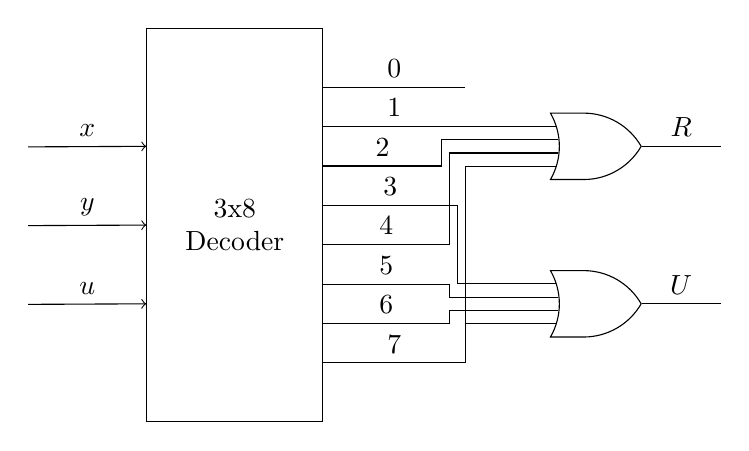
\begin{tikzpicture}
    %coordinates
    \coordinate (orig)   at (0,0);

    \coordinate (Dec) at (1,4);

    \coordinate (x) at ($(Dec) + (-1.5,3.5)$);
    \coordinate (y) at ($(x) + (0,-1)$);
    \coordinate (u) at ($(y) + (0,-1)$);

    %nodes
    \node[draw, minimum width=2cm, minimum height=5cm, anchor=south west, text width=2cm, align=center] (A) at (Dec) {3x8\\Decoder};
    \node[or gate US, draw, logic gate inputs=nnnn] at ($(A)+(4.5,1)$) (B) {};
    \node[or gate US, draw, logic gate inputs=nnnn] at ($(A)+(4.5,-1)$) (C) {};

    %edges
    \draw[->] (x) -- node[above]{$x$} ($(A.180) + (0,1)$);
    \draw[->] (y) -- node[above]{$y$} ($(A.180) + (0,0)$);
    \draw[->] (u) -- node[above]{$u$} ($(A.180) + (0,-1)$);

    \draw ($(A.0) + (0, 1.75)$) -- node[above]{0} ($(A.0) + (1.8, 1.75)$);
    \draw ($(A.0) + (0, 1.25)$) -- node[above]{1} ($(A.0) + (1.8, 1.25)$) |- (B.input 1);
    \draw ($(A.0) + (0, 0.75)$) -- node[above]{2} ($(A.0) + (1.5, 0.75)$) |- (B.input 2);
    \draw ($(A.0) + (0, 0.25)$) -- node[above]{3} ($(A.0) + (1.7, 0.25)$) |- (C.input 1);
    \draw ($(A.0) + (0, -0.25)$) -- node[above]{4} ($(A.0) + (1.6, -0.25)$) |- (B.input 3);
    \draw ($(A.0) + (0, -0.75)$) -- node[above]{5} ($(A.0) + (1.6, -0.75)$) |- (C.input 2);
    \draw ($(A.0) + (0, -1.25)$) -- node[above]{6} ($(A.0) + (1.6, -1.25)$) |- (C.input 3);
    \draw ($(A.0) + (0, -1.75)$) -- node[above]{} ($(A.0) + (1.8, -1.75)$) |- (C.input 4);
    \draw ($(A.0) + (0, -1.75)$) -- node[above]{7} ($(A.0) + (1.8, -1.75)$) |- (B.input 4);

    \draw (C.output) -- node[above]{$U$} ($(C.output) + (1, 0)$);
    \draw (B.output) -- node[above]{$R$} ($(B.output) + (1, 0)$);

    %\draw[->] (A.270) -- node[above]{} (B.90);
    %\draw[->] (C.270) -- node[above]{} (D.90);

    %\draw[->] (A) -| node[above]{} ($(E.180) + (-2,0.3)$) -- node[above]{} ($(E.180) + (0,0.3)$);
    %\draw[->] (B) -| node[above]{} ($(F.180) + (-2,0.3)$) -- node[above]{} ($(F.180) + (0,0.3)$);
    %\draw[->] (C) -| node[above]{} ($(E.180) + (-3,-0.3)$) -- node[above]{} ($(E.180) + (0,-0.3)$);
    %\draw[->] (D) -| node[above]{} ($(F.180) + (-2,-0.3)$) -- node[above]{} ($(F.180) + (0,-0.3)$);

    %\draw[->] (B.270) |- node[above]{} ($(F.180) + (-2.5,+ If I email 0.3)$) |- node[above]{} ($(G.180) + (0,0.3)$);
    %\draw[->] (D.270) |- node[above]{} ($(D.270) + (3.3,-0.5)$) |- node[above]{} ($(G.180) + (0,-0.3)$);

    %\draw[->] (E.270) -- node[above]{} (F.90);
    %\draw[->] (F.270) -- node[above]{} (G.90);

    %\draw[->] (E) -- node[above]{$R_0$} ($(E) + (3, 0)$);
    %\draw[->] (F) -- node[above]{$R_1$} ($(F) + (3, 0)$);
    %\draw[->] (G) -- node[above]{$R_2$} ($(G) + (3, 0)$);
    %\draw[->] (G) |- node[above]{} ($(G) + (0, -2)$) -- node[above]{} ($(G) + (1, -2)$) -- node[above]{$R_3$} ($(G) + (3, -2)$);
  \end{tikzpicture}
\end{center}




\section{Karnaugh Map}
\begin{center}
  %\kvnoindex		% index in boxes
  %\kvunitlength=10mm	% groesse
  \karnaughmap{4}{$f(A,B,C,D):$}{{$A$}{$C$}{$B$}{$D$}}{1100110001001100}
  {
    \put(2,3.5){\color{red}\oval(3.9,0.9)}
    \put(2,4){\color{blue}\oval(1.9,1.9)[b]}
    \put(2,0){\color{blue}\oval(1.9,1.9)[t]}
    \put(3,4){\color{green}\oval(1.9,1.9)[b]}
    \put(3,0){\color{green}\oval(1.9,1.9)[t]}
  }
\end{center}

\begin{align}
  {\color{red}\neg A \neg B} + {\color{blue}\neg B D} + {\color{green}\neg B C}
\end{align}



\section{K2}
\begin{center}
  \karnaughmap{4}{$f(x_1,x_2,x_3,x_4):$}{{$x_1$}{$x_3$}{$x_2$}{$x_4$}}{0010111101DDDDDD}
  {
    \put(3,2){\color{red}\oval(1.9,3.9)}
    \put(4,2){\color{blue}\oval(1.9,1.9)[l]}
    \put(0,2){\color{blue}\oval(1.9,1.9)[r]}
    \put(2,1){\color{green}\oval(1.9,1.9)}
  }
\end{center}

\end{document}
